\section{Results}
\label{sec:results}

Figures \ref{fig:ExeTime_rows} and \ref{fig:ExeTime_columns} show results from the benchmarks that are meant to test theoretical algorithmic complexity of the compression algorithm and its dependence on the size of input matrix. Outcomes are discussed in section Optimization.

\begin{figure}[H]
\centering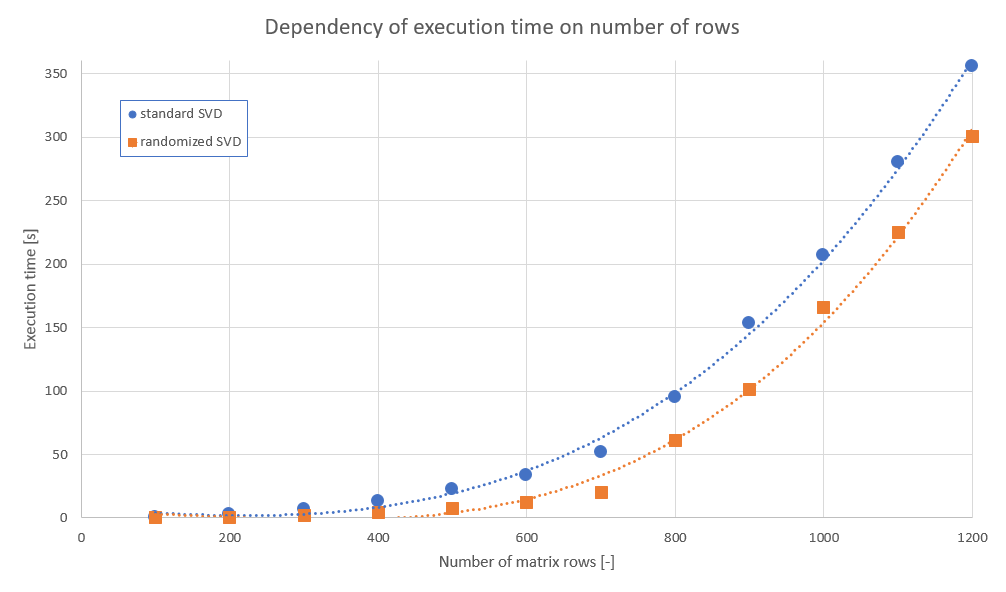
\includegraphics[width=\textwidth]{figures/executionTime_varyingRows}
\caption{Dependency of SVD execution time on number of rows of an input matrix.}
\label{fig:ExeTime_rows}
\end{figure}

\begin{figure}[H]
\centering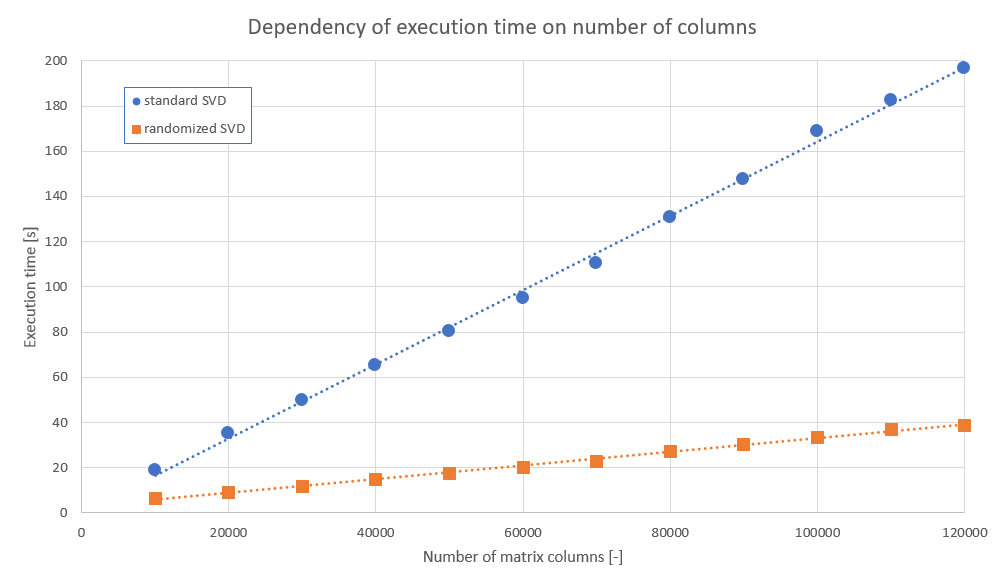
\includegraphics[width=\textwidth]{figures/executionTime_varyingColumns}
\caption{Dependency of SVD execution time on number of columns of an input matrix.}
\label{fig:ExeTime_columns}
\end{figure}

% temelin
In Figure \ref{fig:temelin:mesh}, Figure \ref{fig:chotkova:mesh}, and Figure \ref{fig:mechaxisym:mesh} are depicted visualizations of results of analyses that were used as benchmarks for the compression algorithm. Analyses with distinct character of results were chosen intentionally to cover most cases that can occur in FEM calculations.

Figure \ref{fig:temelin:mesh} shows results from an analysis of aging of nuclear power-plant's containment. This analysis includes high number of analysis steps (thousands) with very little differences between them. There is therefore potential for compression ratio to be very high as proven in Figure \ref{fig:temelin:NRMSD} that examines the impact of changes in the compression ratio to the mean error of approximation.

\begin{figure}[H]
\centering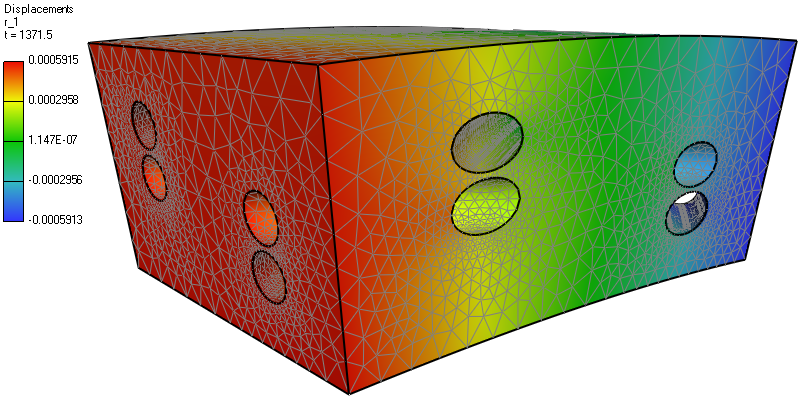
\includegraphics[width=\textwidth]{figures/temelin_screenshot}
\caption{Temelin nuclear power plant. Results visualization (Displacement field, X component).}
\label{fig:temelin:mesh}
\end{figure}

\begin{figure}[H]
\centering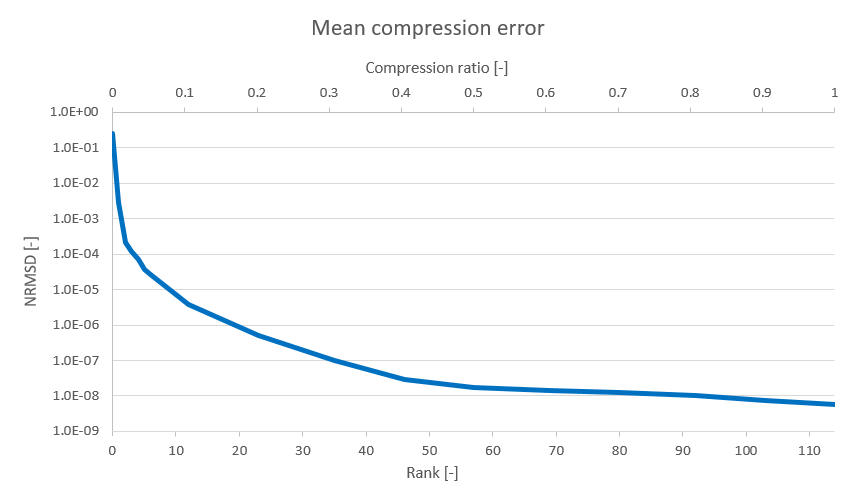
\includegraphics[width=\textwidth]{figures/temelin_NRMSD}
\caption{Dependence of Normalized Rooted Mean Squared Deviation on Compression ratio for Temelin project results.}
\label{fig:temelin:NRMSD}
\end{figure}

% chotkova
Figure \ref{fig:chotkova:mesh} shows results from an analysis of geological layers. This project was chosen mainly to study behavior of compression algorithm when dealing with high discontinuities in data in spatial dimension (as can be seen in visualization). As summarized in Figure \ref{fig:chotkova:NRMSD} and Figure \ref{fig:chotkova:MaxError} this has negligible effect on quality of compression.

\begin{figure}[H]
\centering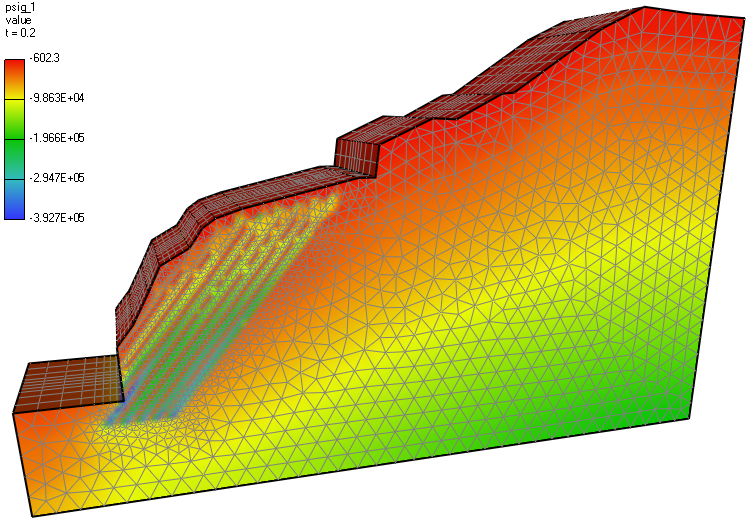
\includegraphics[width=\textwidth]{figures/chotkova_screenshot}
\caption{Chotkova geological layers. Results visualization (Stress field, sigma XX component).}
\label{fig:chotkova:mesh}
\end{figure}

\begin{figure}[H]
\centering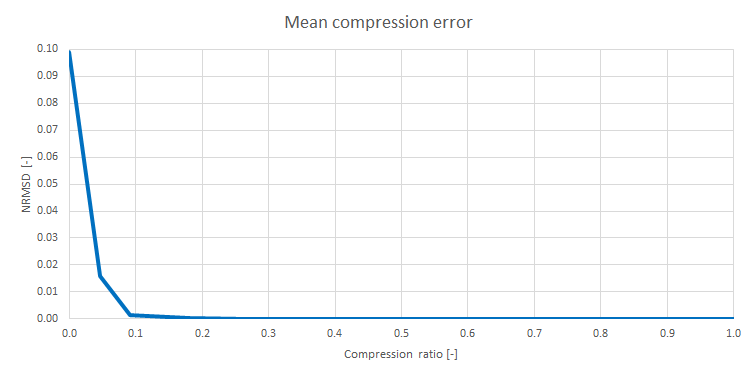
\includegraphics[width=\textwidth]{figures/chotkova_NRMSD}
\caption{Dependence of Normalized Rooted Mean Squared Deviation on Compression ratio for Chotkova project results.}
\label{fig:chotkova:NRMSD}
\end{figure}

\begin{figure}[H]
\centering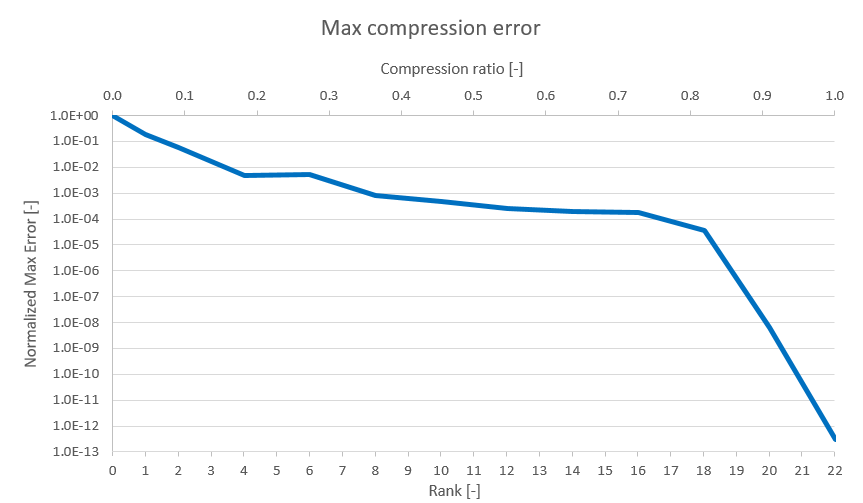
\includegraphics[width=\textwidth]{figures/chotkova_MaxError}
\caption{Dependence of Normalized Maximum Error on Compression ratio for Chotkova project results.}
\label{fig:chotkova:MaxError}
\end{figure}

% mechaxisym
Figure \ref{fig:mechaxisym:mesh} contains visualization of results of two-dimensional analysis. There are exactly 232 analysis steps. The resulting data has linear function character with several discontinuities in temporal dimension. There are few time steps in which resulting discrete functions have very different values compared to neighboring time steps. This was supposed to have negative impact on the quality of compression. However, as can be seen in Figure \ref{fig:mechaxisym:NRMSD}, the quality is better than expected; e.g., if the rank of approximation matrix is set to 3 (compared to 232 being the rank of the original matrix) the normalized relative error (NRMSD) does not exceed $10^{-5}$.

\begin{figure}[H]
\centering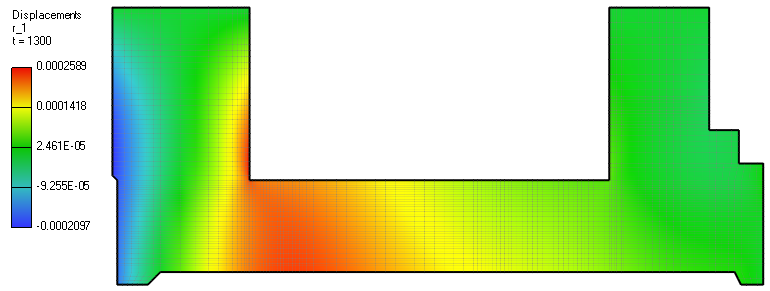
\includegraphics[width=\textwidth]{figures/mechaxisym_screenshot}
\caption{"Mechaxisym" model. Results visualization (displacement field, x component).}
\label{fig:mechaxisym:mesh}
\end{figure}

\begin{figure}[H]
\centering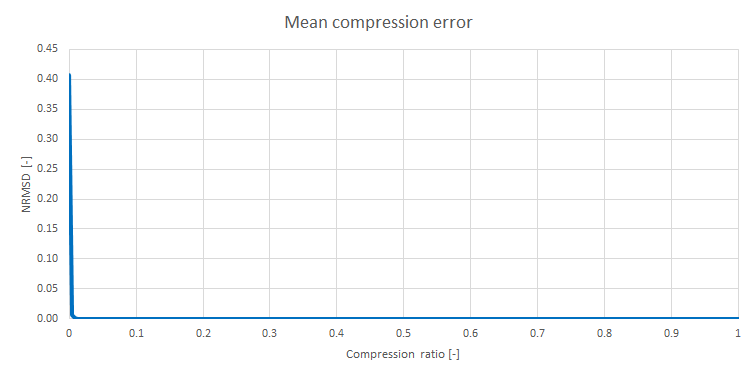
\includegraphics[width=\textwidth]{figures/mechaxisym_NRMSD}
\caption{Dependence of Normalized Rooted Mean Squared Deviation on Compression ratio for Mechaxisym project results.}
\label{fig:mechaxisym:NRMSD}
\end{figure}

% PSNR
Figure \ref{fig:PSNR} summarizes the compression error for all three benchmarks using logarithmic scale to make the differences more visible. Peek signal to noise ratio (PSNR) metric is used (see Equation \ref{eq:psnr-def} for definition). Figure \ref{fig:PSNR_rand} contains the same comparison for the randomized SVD algorithm.

\begin{figure}[H]
\centering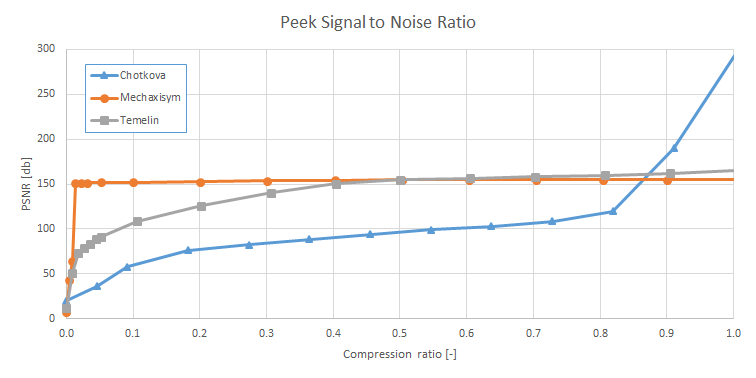
\includegraphics[width=\textwidth]{figures/PSNR}
\caption{Comparison of Peek signal to noise ratio value calculated for different decompositions.}
\label{fig:PSNR}
\end{figure}

\begin{figure}[H]
\centering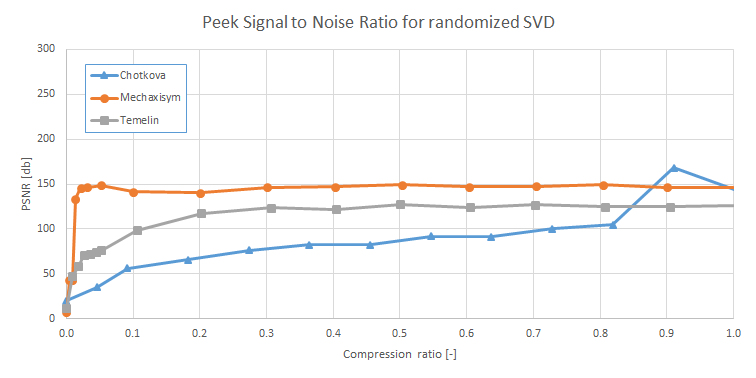
\includegraphics[width=\textwidth]{figures/PSNR_rand}
\caption{Comparison of Peek signal to noise ratio value for different randomized decompositions.}
\label{fig:PSNR_rand}
\end{figure}

% Execution times
Besides the error also the execution speed of compression algorithm was measured. In Figure \ref{fig:temelin:ExeTime} is comparison of execution times for standard versus randomized SVD compression algorithms. Interestingly, execution time of standard SVD is independent of target rank whereas execution time of randomized SVD decreases linearly with decreasing target rank. If the rank is known ahead of time the fact can be taken advantage of.

\begin{figure}[H]
\centering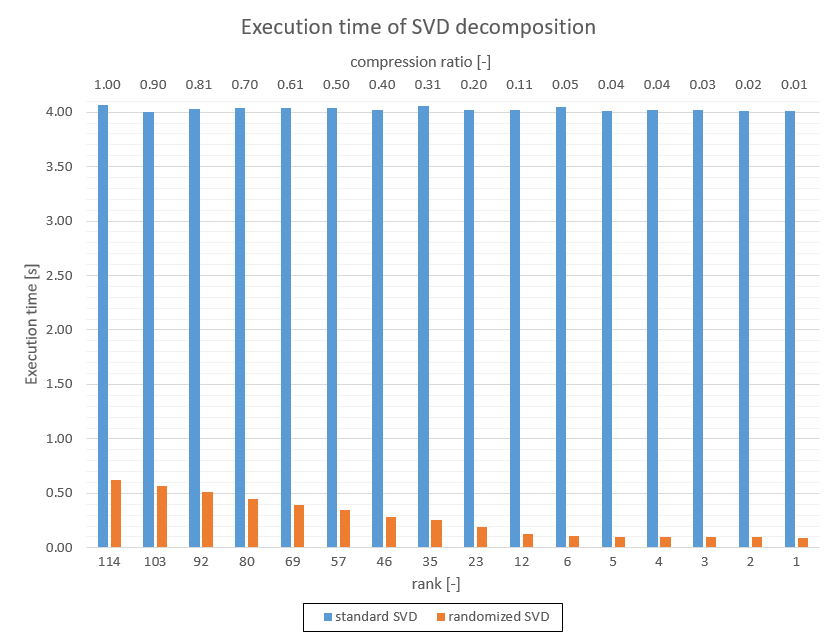
\includegraphics[width=\textwidth]{figures/temelin_ExecutionTime}
\caption{Variation of execution time of standard and randomized decompositions calculated for Temelin analysis results.}
\label{fig:temelin:ExeTime}
\end{figure}

The memory consumption of compressed results for Temelin analysis is summarized in Table \ref{tab:mem-consum}. For different values of compression ratio shows memory size in megabytes. Compression ratio $c$ is an input parameter to the compression algorithm specifying amount of singular values ought to be removed from the SVD decomposition as follows from the equation (\ref{eq:rank-from-comp-ratio}). Size factor describes the final outcome of compression when compared to the original size.

\begin{table}[H]
\centering
    \begin{tabular}{| r | r | r |}
    \hline
    compression ratio ($c$) & memory consumption [MB] & size factor \\ \hline \hline
    1.00 & 2002.1 & 1 \\ \hline
    0.50 & 1006.9 & 0.5002 \\ \hline
    0.10& 211.9 & 0.1053 \\ \hline
    0.01 & 35.3 & 0.0176 \\ \hline
    \end{tabular}
    \caption{Memory consumption of compressed results. Temelin analysis.}
	\label{tab:mem-consum}
\end{table}
